% Template for Cogsci submission with R Markdown

% Stuff changed from original Markdown PLOS Template
\documentclass[10pt, letterpaper]{article}

\usepackage{cogsci}
\usepackage{pslatex}
\usepackage{float}
\usepackage{caption}

% amsmath package, useful for mathematical formulas
\usepackage{amsmath}

% amssymb package, useful for mathematical symbols
\usepackage{amssymb}

% hyperref package, useful for hyperlinks
\usepackage{hyperref}

% graphicx package, useful for including eps and pdf graphics
% include graphics with the command \includegraphics
\usepackage{graphicx}

% Sweave(-like)
\usepackage{fancyvrb}
\DefineVerbatimEnvironment{Sinput}{Verbatim}{fontshape=sl}
\DefineVerbatimEnvironment{Soutput}{Verbatim}{}
\DefineVerbatimEnvironment{Scode}{Verbatim}{fontshape=sl}
\newenvironment{Schunk}{}{}
\DefineVerbatimEnvironment{Code}{Verbatim}{}
\DefineVerbatimEnvironment{CodeInput}{Verbatim}{fontshape=sl}
\DefineVerbatimEnvironment{CodeOutput}{Verbatim}{}
\newenvironment{CodeChunk}{}{}

% cite package, to clean up citations in the main text. Do not remove.
\usepackage{cite}

\usepackage{color}

% Use doublespacing - comment out for single spacing
%\usepackage{setspace}
%\doublespacing


% % Text layout
% \topmargin 0.0cm
% \oddsidemargin 0.5cm
% \evensidemargin 0.5cm
% \textwidth 16cm
% \textheight 21cm

\title{Word Learning as Network Growth: A Cross-linguistic Analysis}

\usepackage{tipa}

\author{{\large \bf Abdellah Fourtassi} \\ \texttt{afourtas@stanford.edu} \\ Department of Psychology \\ Stanford University \And {\large \bf Yuan Bian} \\ \texttt{ybian.uiuc@gmail.com} \\ Department of Psychology \\ University of Illinois \And {\large \bf Michael C. Frank} \\ \texttt{mcfrank@stanford.edu} \\ Department of Psychology \\ Stanford University}

\begin{document}

\maketitle

\begin{abstract}
Stager and Werker (1997) first showed that chidlren's early ability to
distinguish similar sounds do not automatically translate into word
learning skills. Early explanations proposed that children may not be
able to encode subtile phonetic contrasts when learning novel word
meanings, thus suggesting a binary/discontinuous pattern of development.
However, later work has revealed (e.g., through using simpler testing
methods) that children do encode such contrasts, thus favoring a rather
probabilitic/continuous pattern of development. The present study
proposes a precise probabisitic model describing how development may
processd in a continuous fashion. The purpose of the model is to account
for previousely documented facts while providing new predictions. We
collected data from both preschool children and adults, and we show that
the model can explain various patterns of learning both within the same
age and across development. More generally, our work highlight the role
of computational modeling in advancing our understanding of development
through both organizing exsinting knowledge and generating new
principled hypotheses.

\textbf{Keywords:}
word learning, cogniive development, computational modeling
\end{abstract}

\section{Introduction}\label{introduction}

Over the first year of life, children become sensitive to the phonetic
variations that are used to distinguish meanings in their native
language (Werker \& Tees, 1984). One could imagine that these perceptual
skills would be automatically applied to the task of word learning.
However, developmental data show that 14 m.o children find it
challenging to associate minimally different (but perceptually
discriminated) sounds such as ``bin'' and ``din'' to different objects
(Stager \& Werker, 1997).

Several factors can explain this finding. For example it is possible
that the task of meaning learning increases cognitive demands on
children (compared to a simple perceptual descrimination). In
particular, it requires paying attention to both the sounds and the
corresponding objects, which may hinder precise encoding in memory of
some phonetic details (Hofer \& Levy, 2017; Stager \& Werker, 1997).
Additional difficulty might arise from ambiguous phonological boundaries
at this stage of development (e.g., Rost \& McMurray, 2009), or from
uncertainty about the referential status of the novel word (Fennell \&
Waxman, 2010).

Regardless of the exact explanation, it is generally accepted that by
around 17 m.o, chidlren succeed under the same circumstances (Werker,
Fennell, Corcoran, \& Stager, 2002). What could be the mechanism of
development? On one possible account, learning is stage-like: younger
children learn a single, underspecified representation of similar words
(e.g., ``bin''/``din''). Development occurs when children specify this
intial coarse reprepsentation and learn two distinct catgories. On an
other account, learning is continuous: distinct represetations are
learned even by younger children, but these representations are encoded
with higher uncertainty in youger children, leading to apparent failure
in relatively demanding tasks. Development is a continuous process
whereby the intinial noisy representations become more precise (see
also, Swingley, 2007).

Experimental evidence suggest a probabilsitic/continuous, rather than a
binary/discontinuous develomental scenario. On the one hand,
14-month-olds who typically fail in the original task succeed both when
an easier testing method is used (Yoshida, Fennell, Swingley, \& Werker,
2009), and when uncertainty is mitigated via disambiguating cues
(Dautriche, Swingley, \& Christophe, 2015; Thiessen, 2007). On the other
hand, adults show patterns of learning similar to those shown by
14-month-olds when the task is more challenging and when similarity
between words increases (Pajak, Creel, \& Levy, 2016; White, Yee,
Blumstein, \& Morgan, 2013).

Here talk about the continuous hypothesis a bit later here. after
introducing the experimental evidecne.

Also talk more about the major assumption of model, what is contiuous
about him? and what is the source of this hypothsis (swingley, Yoshida,
\ldots{})

In the light of these evidence, the purpose of the current work is to
propose a precise probabilsitc model of the Stager and Werker's task
where developmment is understood to proceed in a continuous fashion
across the lifespan. We use this model to both provide a unifying
account for documented experimental findings, and to make new
predicitions that have not been tested before. Using new data collected
from both preschool children and adults, we show that the model can
explain various patterns of learning both within the same age and across
development.

\section{Model}\label{model}

\subsection{Task}\label{task}

We model the word learning task introduced by Stager \& Werker (1997),
and a testing method similar to the one used by Yoshida et al. (2009).
In this task, particiants are first exposed to the association between
pairs of nonesense words (e.g., ``lif''/``neem'') and pairs of objects.
After this exposure phase, participants perform a series of
two-alternative forced choices. In each testing trial, one of the two
sounds is uttered (e.g., ``lif'') and participants choose the
corresponding object from the two alternatives. An overview of the task
is shown in Figure~@ref(fig:task).

\begin{CodeChunk}
\begin{figure}[t]

{\centering 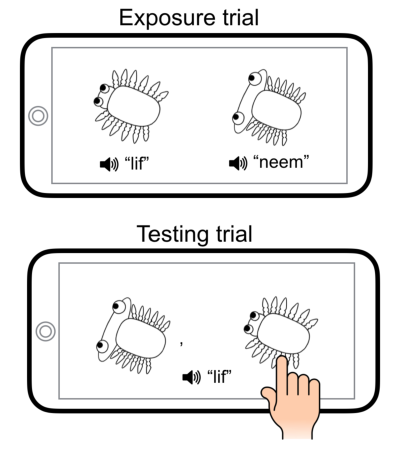
\includegraphics{figs/task-1} 

}

\caption{\label{fig:task}An overview of the task used in this study.}\label{fig:task}
\end{figure}
\end{CodeChunk}

\subsection{Probabilistic strcuture}\label{probabilistic-strcuture}

Our model consists of a set of variables describing the general process
of spoken word recognition in a referential situation. These variables
are related in a way that refelects the simple generative scenario
represented graphically in Figure~@ref(fig:model). When a speaker utters
a sound in the presence of an object, the observer assumes that the
object \(o\) activated the concept \(C\) in the speaker's mind. The
concept prompted the cooresponding label \(L\). Finally, the label was
physically instantiated by the sound \(s\).

A similar probabilsitic structure was used by Lewis \& Frank (2013) to
model concept learning, and by Hofer \& Levy (2017) to model spoken word
learning. However, the first study assumed that the sounds are heard
unambiguousely, and the second assumed the concepts are observed
unambiguously. In our model, we made the more reaistic assumption of
ambiguity at the level of both the sounds and the objects. For
simplicity, we assume that the probability of membership of objects and
sounds to concepts and labels, respectively, are normally distributed:

\[ p(o | C) \sim  \mathcal{N}(\mu_C, \sigma^2_C) \]
\[ p(s| L) \sim  \mathcal{N}(\mu_L, \sigma^2_L) \] We assume there to be
one-to-one mappings between concepts and labels, and that observers have
successfully learned these mappings during the exposure phase: \[
P(L_i|C_j) = 
\begin{cases}
  1 & \text{if  }  i=j \\  
  0  & \text{if  }  i\neq j 
\end{cases}
\]

\subsection{Simulations}\label{simulations}

During the testing phase, participants are presented with one target
sound \(s_T \in\{s_1, s_2\}\) and the two objects \(o_1\) and \(o_2\)
presented during the learning phase. In order to make a choice, we
determine which object is more probable under the target sound \(s_T\),
in other words, we compare the the probabilities \(P(o_1|s_T)\) and
\(P(o_2|s_T)\). The values of these probabilities can be computed by
summing over all possible concepts and labels:
\[P(o|s)=\sum_{C,L} P(o, C, L| s) \propto \sum_{C,L} P(o, C, L, s) \]
The joint probability \(P(o, C, L, s)\) is obtained by factoring the
bayesian network in Figure 2: \[P(o,C,L,s) = P(s|L)P(L|C)P(C|o)P(o) \]
which could be tansformed using Bayes rule into:

\[P(o,C,L,s) = P(s|L)P(L|C)P(o|C)P(C) \] Finally, assuming that the
concept prior probability is uniformly ditributed, we obtain the
following expression, where all conditional dependencies have been
defined in the previous sub-section.

\begin{equation}
P(o|s) = \frac{\sum_{C,L} P(s|L)P(o|C)P(L|C)}{\sum_{o} \sum_{C,L} P(s|L)P(o|C)P(L|C)}
\end{equation}

From the general expression (1) we derive the exact analytical formula
which expresses the probability of accurate responses in the testing
phase (Figure 1).

\begin{equation}
P(o_T|s_T)= \frac{1 + e^{-(\Delta s^2 + \Delta o^2) /2\sigma^2}}{1 + e^{-(\Delta s^2 + \Delta o^2) /2\sigma^2} + e^{-\Delta s^2 /2\sigma^2} + e^{-\Delta o^2 /2\sigma^2 }}
\end{equation}

\begin{CodeChunk}
\begin{figure}[h]

{\centering 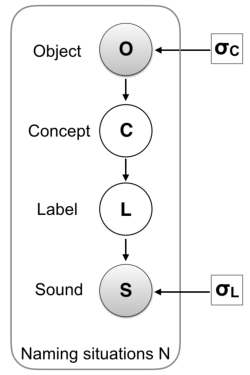
\includegraphics{figs/model-1} 

}

\caption{\label{fig:model}Graphical representation of our model. Circles indicate random variables (shading indicates observed variables). The squares indicates fixed model parameters.}\label{fig:model}
\end{figure}
\end{CodeChunk}

We provide an intuitive illustration of how this probabilistic account
explain patterns of learning and development in Figure XX. Low accuracy
in word learning occurs when the perceptual distance between the labels
is small relative to the uncertainty with wich these labels are encoded.
For example, in Stager and Werker's orginal experiment, children are
supposed to associate lable 1 (``bih'') and label 2 (``dih'') with
object 1 and object 2, respectively. Though children could learn that
the label ``bih'' is a better match to object 1 than ``dih'', they could
still judge the sound ``dih'' as a plausible instance of the lable
``bih'', thanks to the relatively large variance/tolerance of the
encoding.

Accuracy is high when the perceptual distance between the labels is
large relative to the uncertainty of their encoding. Thus, improvement
can occur in the same developmental stage if the perceptual distance of
the labels is enhanced either through using different-sounding labels
(e.g., ``lif'' vs. ``neem'' instead of ``bih'' and ``dih'') or through
using additional disambiguating cues (e.g., Thiessen, 2007). Accuracy
improves over development because the encoding's uncertainty itself is
reduced.

In order to have a more quantitative understanding of the mdoel, we
simulate the values of the predicted accuracy (Expression 2) as a
function of the perceptual distance between the sounds \(\Delta s\). We
used as parameters the two remaning variables, i.e., the visual distance
between the semantic referents \(\Delta o\) and the standard deviation
of the dsitributions \(p(s| L)\) and \(p(o | C)\) (which, in this
simulation, have similar values, i.e.,
\(\sigma =\sigma_C \approx \sigma_L\)). The simulations are shown in
Figure 3.

\begin{CodeChunk}
\begin{figure*}[h]

{\centering 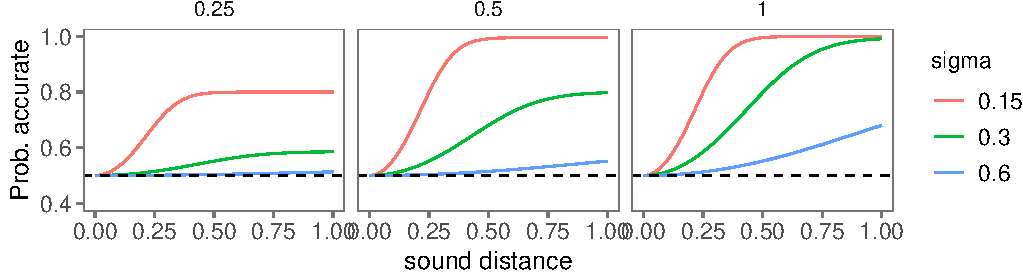
\includegraphics{figs/simulation-1} 

}

\caption{\label{fig:simulation}The predicted probability of accurate responses in the task of learning two similar-sounding words, as a function the perceptual distance between the sounds. Colors indicate different values of the standard deviation which we assume is common to both the label and concept probabilistic representations. Panels represent graphs using different values of the visual distance between the objects.}\label{fig:simulation}
\end{figure*}
\end{CodeChunk}

The simulations explain previousely documented facts, and make new
predictions:

\begin{enumerate}
\def\labelenumi{\arabic{enumi})}
\item
  For fixed values of \(\Delta o\) and \(\sigma\), the probability of
  accurate responses increases as a function of \(\Delta s\). This
  pattern accounts for the fact that similar sounds are generally more
  challenging to learn than different sounds for both chidlren (Stager
  \& Werker, 1997) and adults (Pajak et al., 2016).
\item
  For fixed values of \(\Delta s\) and \(\Delta o\), accuracy increases
  when the representational noise (characterized with \(\sigma\))
  decreases. This fact may explain development, i.e., youger children
  have noisier representations (Swingley, 2007; Yoshida et al., 2009),
  which leads to lower word recognition accuracy, especially for similar
  sounding words.
\item
  For fixed values of \(\Delta s\) and \(\sigma\), accuracy increases
  with the visual distance between the semantic referents \(\Delta o\).
  This is a new predcition that our model makes. Previous work studied
  the effect of several bottom-up and top-down properties in
  disambiguating similar sounding words (Dautriche et al., 2015; Fennell
  \& Waxman, 2010; Rost \& McMurray, 2009; Thiessen, 2007), but no
  previous study tested the effect of the visual distance between the
  semantic referents.
\end{enumerate}

To sum, we introduced a model that accounts for some qualitative
learning patterns observed in previous studies, and makes a new
prediction. In the experiment below, we test whether the model makes
accurate \emph{quantitative} predictions by fitting it to new
experimental data collected from preschool chidlren and adults.

\begin{CodeChunk}
\begin{figure}[H]

{\centering 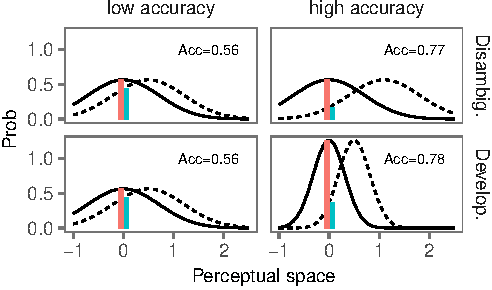
\includegraphics{figs/illus-1} 

}

\caption{\label{fig:illus} An illustration of how a probabilsitic account (where distinct categories are encoded with different degrees of uncertainty) can explain patterns of learning and development. Accuracy experesses the extent to which a given sound instance indicates a unique category. The values vary between 0.5 (total overlap) and 1 (no overalp). Accuracy is low when the perceptual distance between labels is small relative to the category variance. Accuracy increases when the perceptual distance is enhanced (through disambiguation), or when the variance decreases (e.g., through development).}\label{fig:illus}
\end{figure}
\end{CodeChunk}

\section{Experiment}\label{experiment}

In this experiment, we tested participants in the word learning task
introduced above (Figure 1). We explored all three parameters of the
model. Both the sound similarity (\(\Delta s\)) and object similarity
(\(\Delta o\)) were varied simulataneousely in a within-subject design.
Besides, two age groups (preschool children and adults) were tested on
the same task to explore whether development can be characteized with
the degree of uncertainty, \(\sigma\), in the probabilsitic
representations.

\subsection{Methods}\label{methods}

\subsubsection{Participants}\label{participants}

We planned to recruit a sample of 60 children ages 4-5 years from the
Bing Nursery School on Stanford University's campus. So far, we
collected data from N=47 children (mean age= months, F=). An additional
28 children participated but were removed from analyses because they
were not above chance on the catch trials (as was specified in the
pre-registration\footnote{https://osf.io/jrh38/}). We also collected a
planed sample of N=30 adults on Amazon Mechanical Turk. N=2 adult
participants were excluded because of low scores on the catch trials
(see pre-registration).

\subsubsection{Stimuli and similarity
rating}\label{stimuli-and-similarity-rating}

The sound stimuli were generated using the MBROLA Speech Synthesizer
(Dutoit, Pagel, Pierret, Bataille, \& Van der Vrecken, 1996). We
generated three kinds of sound pairs which varied in their degree of
similarity to English speakers: 1) ``different'': ``lif''/``neem'' and
``zem''/``doof'', 2) ``intermediate'': ``aka''/``ama'' and
``ada''/``aba'', and 3) ``similar'' non-English minimal pairs:
``ada''/``a\textipa{d\super h}a'' (in hindi) and
``a\textipa{Q}a''/``a\textipa{\textcrh}a'' (in arabic).

As for the objects, we used the Dynamic Stimuli javascript
library\footnote{https://github.com/erindb/stimuli} which allowed us to
generate objects in four different categories: ``tree'', ``bird'',
``bug'', and ``fish''. These categories are supposed to be naturally
occuring kinds that might be seen on an alien planet. In each category,
we generated ``different'', ``intermediate'' and ``similar'' levels of
similarity by manipuating a continuous property controling features of
the category's shape (e.g, body strech and head fatness).

In a separate survey, \(N=20\) participants recruited on Amazon
Mechanical Turk evaluated the similarity of each sound and objcet pair
on a 7-point scale. We computed averge ratings across partcipants, and
we normalized the data so that the values vary between 0 to 1. Results
are shown in Figure XX, for each stimuli group. This data will be used
in the models as the perceptual distance of sound pairs (\(\Delta s\))
and object pairs (\(\Delta o\)).

\begin{CodeChunk}
\begin{figure}[h]

{\centering 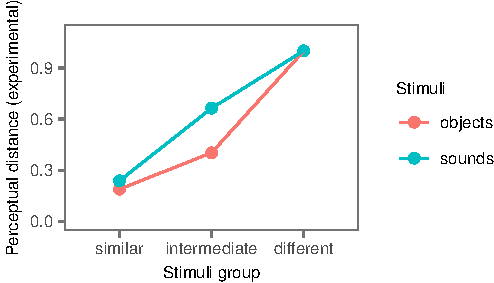
\includegraphics{figs/stim-1} 

}

\caption{\label{fig:stim}Normalized distances for both sound and object pairs used in this study.}\label{fig:stim}
\end{figure}
\end{CodeChunk}

\subsubsection{Design}\label{design}

Each age group saw only two of the three levels of similarity described
in the previous sub-section: ``different'' vs. ``intermediate'' for
preschoolers, and ``intermediate'' vs. ``similar'' for adults. The
experiment consisted of four conditions which involved, each, one pair
of sounds-objects associations. These conditions were constructed by
crossing the sound's degree of similarity with the object's degree of
similarity leading to a 2x2 factorial design in each age group. Besides
the 4 conditions, we also tested participants on a fifth catch condition
which was similar in its stucture to the other ones, but was used only
to select participant who were able to follow the instructions and show
minimal learning.

\begin{CodeChunk}
\begin{figure*}[h]

{\centering 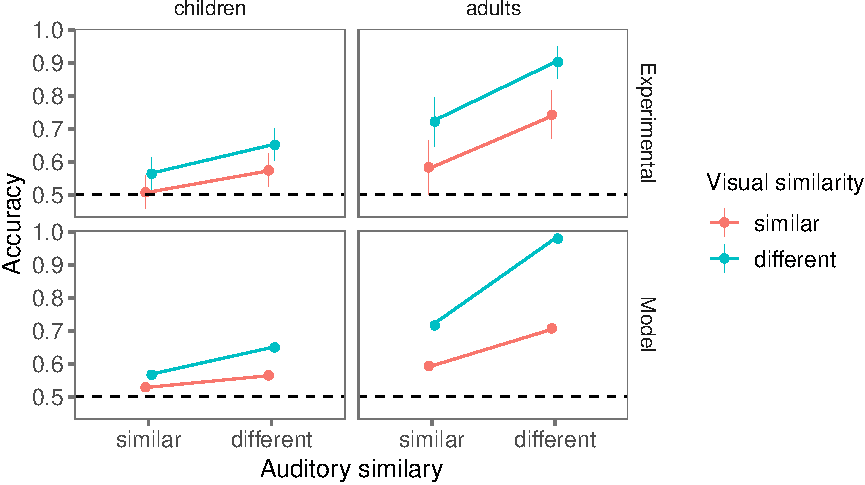
\includegraphics{figs/all_data-1} 

}

\caption{\label{fig:data_all}Accuracy of novel word recognition as as a function of the sound distance, the object distance, and the age group (preschool children vs. Adults). Experimental results are shown on the left. Predictions from Model 1 (one free parameter) and Model 2 (two free parameters) are shown in the middle and on the right, respectively.}\label{fig:all_data}
\end{figure*}
\end{CodeChunk}

\subsubsection{Procedure}\label{procedure}

Preschoolers were asked if they would be willing to play a game on a
tablet with the experimenter and were informed that they could stop
playing at any time. The experimenter explained that the game consisted
in learning some words spoken in an alien planet. The experiment began
with two simple examples (not included in the analysis), and in these
examples children were given feedback from the experimenter so as to
make sure they correctly understood the structure of the task. After the
introduction and examples, children were tested in a sequence of five
conditions: the four experimental conditions plus the catch condition.
In each condition, participants saw a first block of four exposure
trials followed by four testing trials, and a second block of two
exposure trials (for memory refreshment) follwoed by an additional four
testing trials.

In the exposure trials, children saw two objects associated with their
corresponding sounds. We presented the first object on the left side of
the tablet's screen simultaneously with the corresponding sound. The
second sound-object association followed on the other side of the screen
after 500ms. For both objects, visual stimuli were present for the
duration of the sound clip (∼800ms). In the testing trials, children saw
both objects simultaneousely and heard only one sound. They completed
the trial by selecting which of the two objects corresponded to the
sound. They responded by touching one of the pictures on the tablet.

The object-sound pairings were randomized across participants, as was
the order of the conditions (except for the catch condition which was
always placed in the middle of the testing sequence). We also randomized
the on-screen position (left vs.~right) of the two pictures on each
testing trial.

The procedure for preschoolers and adults were identical except that
preschoolers were accompagnied by an experimenter and used a tablet,
whereas adults used their local computers to complete the experiment
online.

\subsubsection{Model fitting}\label{model-fitting}

We fit the analystical expression (equation 2) to the participants'
responses in each age group. The values of \(\Delta s\) and \(\Delta o\)
were set based on data from the similarity judgment task (described in
the stimuli sub-section). We used two models: \textbf{model 1} fit only
one parameter (\(\sigma = \sigma_C =\sigma_L\)), and \textbf{model 2}
fit two parameters (\(\sigma_C \neq \sigma_L\)). The values of the
parameters were derived using weighted least-squares estimates.

\subsection{Results}\label{results}

First we analyzed the experimental results shown in Figure (XX, left),
using a mixed-effects logistic regression with sound and object
distances as fixed effects, and with a maximal random effects strcuture
(Barr, Levy, Scheepers, \& Tily, 2013). Results are shown in Table XX.
We found a main effect of sound distance on the accuray of learning in
both children and adults, thus replicating previous findings. We also
found a main effect of object distance, thus confirming the new
prediction of our model.

\begin{table}[!htbp] \centering 
  \caption{Estimates of predictor coefficients (and their standard errors) by age group in the regression model} 
  \label{} 
\begin{tabular}{@{\extracolsep{5pt}}lcc} 
\\[-1.8ex]\hline \\[-1.8ex] 
 & Children & Adults \\ 
\hline \\[-1.8ex] 
 (Intercept) & 0.426$^{*}$ (0.199) & 3.114$^{**}$ (1.015) \\ 
  Sound  & 0.272$^{**}$ (0.100) & 2.320$^{*}$ (0.981) \\ 
  Object & 0.315$^{*}$ (0.137) & 2.133$^{*}$ (0.952) \\ 
  Sound x Object & 0.151 (0.097) & 1.821 (0.976) \\ 
 \hline \\[-1.8ex] 
\textit{Note:}  & \multicolumn{2}{r}{$^{*}$p$<$0.05; $^{**}$p$<$0.01; $^{***}$p$<$0.001} \\ 
\end{tabular} 
\end{table}

Figures XX (middle and right graphs) show the predictions of the models.
Both model 1 and model 2 fit reseanaby well the experimental data in
both children and adults. In particular, they both correcly predict the
relative recognition accuacy accross conditions: the pair of words that
differ on both the object and sound levels were the easiest to learn,
followed by the pairs of words that differ on only one level, then the
pair of words that are similar on both levels.

For Model 1, the fitted noise parameter was \(\sigma =\) 0.63 {[}0.53,
0.73{]} for preschoolers, and \(\sigma =\) 0.16 {[}0.12, 0.19{]} for
adults. It explained the majority of the variance (\(R^2=\) 0.94). For
model 2, children had a sound specific noise of \(\sigma_S =\) 0.9
{[}0.68, 1.11{]}, and a concept specific noise of \(\sigma_C =\) 0.29
{[}0.1, 0.49{]}. Adults had a sound specific noise of \(\sigma_S =\)
0.16 {[}0.05, 0.28{]}. The model explain almost all the variance
(\(R^2=\) 0.96), and a concept specific noise of \(\sigma_C =\) 0.14
{[}0.05, 0.23{]}. Note that, despite the fact that Model 1 used only one
degree of freedom, it captures the data variance almost as well as Model
2 which used two degrees of freedom.

\section{General Discussion}\label{general-discussion}

Here maybe be more precise about what the model does (providing a
summary in prose of the main results )

Subsequent studies have shown that To account for this phenomenon, we
proposed a model where words and their semantic referents are both
encoded in a probabilistic fashion. A pair of words may be encoded
simultaneousely, but successful recognition depends both on the
perceptual distance between the words and on the degree of uncertainty
of their encoding. These predictions explained learning patterns both
within and across developmental stages, respectively.

Besides accounting for previous findings, our model made a new
prediction: learning similar words is not only modulated by to
similarity of their phonological forms, but also by the visual
similarity of their semantic referents. More generally, since visual
similarity is an early organizing feature in the semantic domain (e.g.,
Wojcik \& Saffran, 2013), our finding suggest that children may
prioritize the acqusition of words that are quite distant in the
semantic space. This suggestion is supported by recent findings based on
the investigation of early vocabulary growth (Engelthaler \& Hills,
2017; Sizemore, Karuza, Giusti, \& Bassett, 2018). That said, further
work is needed to explore the effect on word learning of other semantic
dimensions that could be encoded by children (e.g.,
conceptual/functional features).

Our model can be seen as an ideal observer (Anderson, 1990) in the sense
that it provides a precise charaterization of the task, and shows how
information can used optimally to perform this task. In our case, the
input is categorized with uncertainty, thus the model performs an
optimal probabilistic (Bayesian) inference, combining cues from both the
sound and the semantic referents. Crucially, we assume the degree of
this uncertainty to vary across development. Thus, although children and
adults appear to behave differently, they are both near-optimal with
resprect to their own encoding's uncertainty. Note that our model is
agnostic as to the precise source of this uncertainty: part of it maybe
due to ambiguous phonological boundaries ({\textbf{???}}), and another
part could be due to various task demands ({\textbf{???}}).

To conclude, this study proposed a model of novel word is compatible
with the hypothesis according to which development is not so much about
a qualitative cognitive change as much as it is about the quantitative
refinement of similar skills acrss the lifespan (Pajak et al., 2016;
Swingley, 2007; Yoshida et al., 2009).

Discuss Hofer \& Levy, 2017, and Fourtassi \& Frank, 2017

\vspace{1em}

\fbox{\parbox[b][][c]{7.3cm}{\centering All data and code for these analyses are available at\ \url{https://github.com/afourtassi/networks}}}
\vspace{1em}

\section{Acknowledgements}\label{acknowledgements}

This work was supported by a post-doctoral grant from the Fyssen
Foundation, NSF \#1528526, and NSF \#1659585.

\section{References}\label{references}

\setlength{\parindent}{-0.1in} \setlength{\leftskip}{0.125in} \noindent

\hypertarget{refs}{}
\hypertarget{ref-anderson1990}{}
Anderson, J. R. (1990). \emph{The adaptive character of thought}.
Hillsdale, NJ: Erlbaum.

\hypertarget{ref-barr2013}{}
Barr, D., Levy, R., Scheepers, C., \& Tily, H. (2013). Random effects
structure for confirmatory hypothesis testing: Keep it maximal.
\emph{Journal of Memory and Language}, \emph{68}(3).

\hypertarget{ref-dautriche2015}{}
Dautriche, I., Swingley, D., \& Christophe, A. (2015). Learning novel
phonological neighbors: Syntactic category matters. \emph{Cognition},
\emph{143}.

\hypertarget{ref-dutoit1996}{}
Dutoit, T., Pagel, V., Pierret, N., Bataille, F., \& Van der Vrecken, O.
(1996). The mbrola project: Towards a set of high quality speech
synthesizers free of use for non commercial purposes. In
\emph{Proceedings of ICSLP} (Vol. 3). IEEE.

\hypertarget{ref-engelthaler2017}{}
Engelthaler, T., \& Hills, T. T. (2017). Feature biases in early word
learning: Network distinctiveness predicts age of acquisition.
\emph{Cognitive Science}, \emph{41}.

\hypertarget{ref-fennell2010}{}
Fennell, C., \& Waxman, S. (2010). What paradox? Referential cues allow
for infant use of phonetic detail in word learning. \emph{Child
Development}, \emph{81}.

\hypertarget{ref-hofer2017}{}
Hofer, M., \& Levy, R. (2017). Modeling Sources of Uncertainty in Spoken
Word Learning. In \emph{Proceedings of the 39th Annual Meeting of the
Cognitive Science Society}.

\hypertarget{ref-lewis2013}{}
Lewis, M., \& Frank, M. (2013). An integrated model of concept learning
and word-concept mapping. In \emph{Proceedings of the annual meeting of
the cognitive science society} (Vol. 35).

\hypertarget{ref-pajak2016}{}
Pajak, B., Creel, S., \& Levy, R. (2016). Difficulty in learning
similar-sounding words: A developmental stage or a general property of
learning? \emph{Journal of Experimental Psychology: Learning, Memory,
and Cognition}, \emph{42}(9).

\hypertarget{ref-rost2009}{}
Rost, G. C., \& McMurray, B. (2009). Speaker variability augments
phonological processing in early word learning. \emph{Developmental
Science}, \emph{12}.

\hypertarget{ref-sizemore2018}{}
Sizemore, A. E., Karuza, E. A., Giusti, C., \& Bassett, D. S. (2018).
Knowledge gaps in the early growth of semantic feature networks.
\emph{Nature Human Behaviour}, \emph{2}(9).

\hypertarget{ref-stager1997}{}
Stager, C., \& Werker, J. (1997). Infants listen for more phonetic
detail in speech perception than in word-learning tasks. \emph{Nature},
\emph{388}(6640).

\hypertarget{ref-swingley2007}{}
Swingley, D. (2007). Lexical exposure and word-form encoding in
1.5-year-olds. \emph{Developmental Psychology}, \emph{43}(2).

\hypertarget{ref-thiessen2007}{}
Thiessen, E. (2007). The effect of distributional information on
children's use of phonemic contrasts. \emph{Journal of Memory and
Language}, \emph{56}.

\hypertarget{ref-werker1984}{}
Werker, J., \& Tees, R. (1984). Cross-language speech perception:
Evidence for perceptual reorganization during the first year of life.
\emph{Infant Behavior and Development}, \emph{7}.

\hypertarget{ref-werker2002}{}
Werker, J., Fennell, C., Corcoran, K., \& Stager, C. (2002). Infants'
ability to learn phonetically similar words: Effects of age and
vocabulary size. \emph{Infancy}, \emph{3}.

\hypertarget{ref-white2013}{}
White, K., Yee, E., Blumstein, S., \& Morgan, J. (2013). Adults show
less sensitivity to phonetic detail in unfamiliar words, too.
\emph{Journal of Memory and Language}, \emph{68}(4).

\hypertarget{ref-wojcik2013}{}
Wojcik, E., \& Saffran, J. (2013). The ontogeny of lexical networks:
Toddlers encode the relationships among referents when learning novel
words. \emph{Psychological Science}, \emph{24}(10).

\hypertarget{ref-yoshida2009}{}
Yoshida, K., Fennell, C., Swingley, D., \& Werker, J. (2009).
14-month-olds learn similar-sounding words. \emph{Developmental
Science}, \emph{12}.

\end{document}
